\chapter{Data-MC comparison for the electroweak analysis}
\label{app:ewk:datamc}

This appendix contains the data-MC comparison for the analysis variables not shown in Chapter \ref{chap:ewk_prod}.

\begin{figure*}[htbp]
\centering 
\subfigure[\pt leading jet]{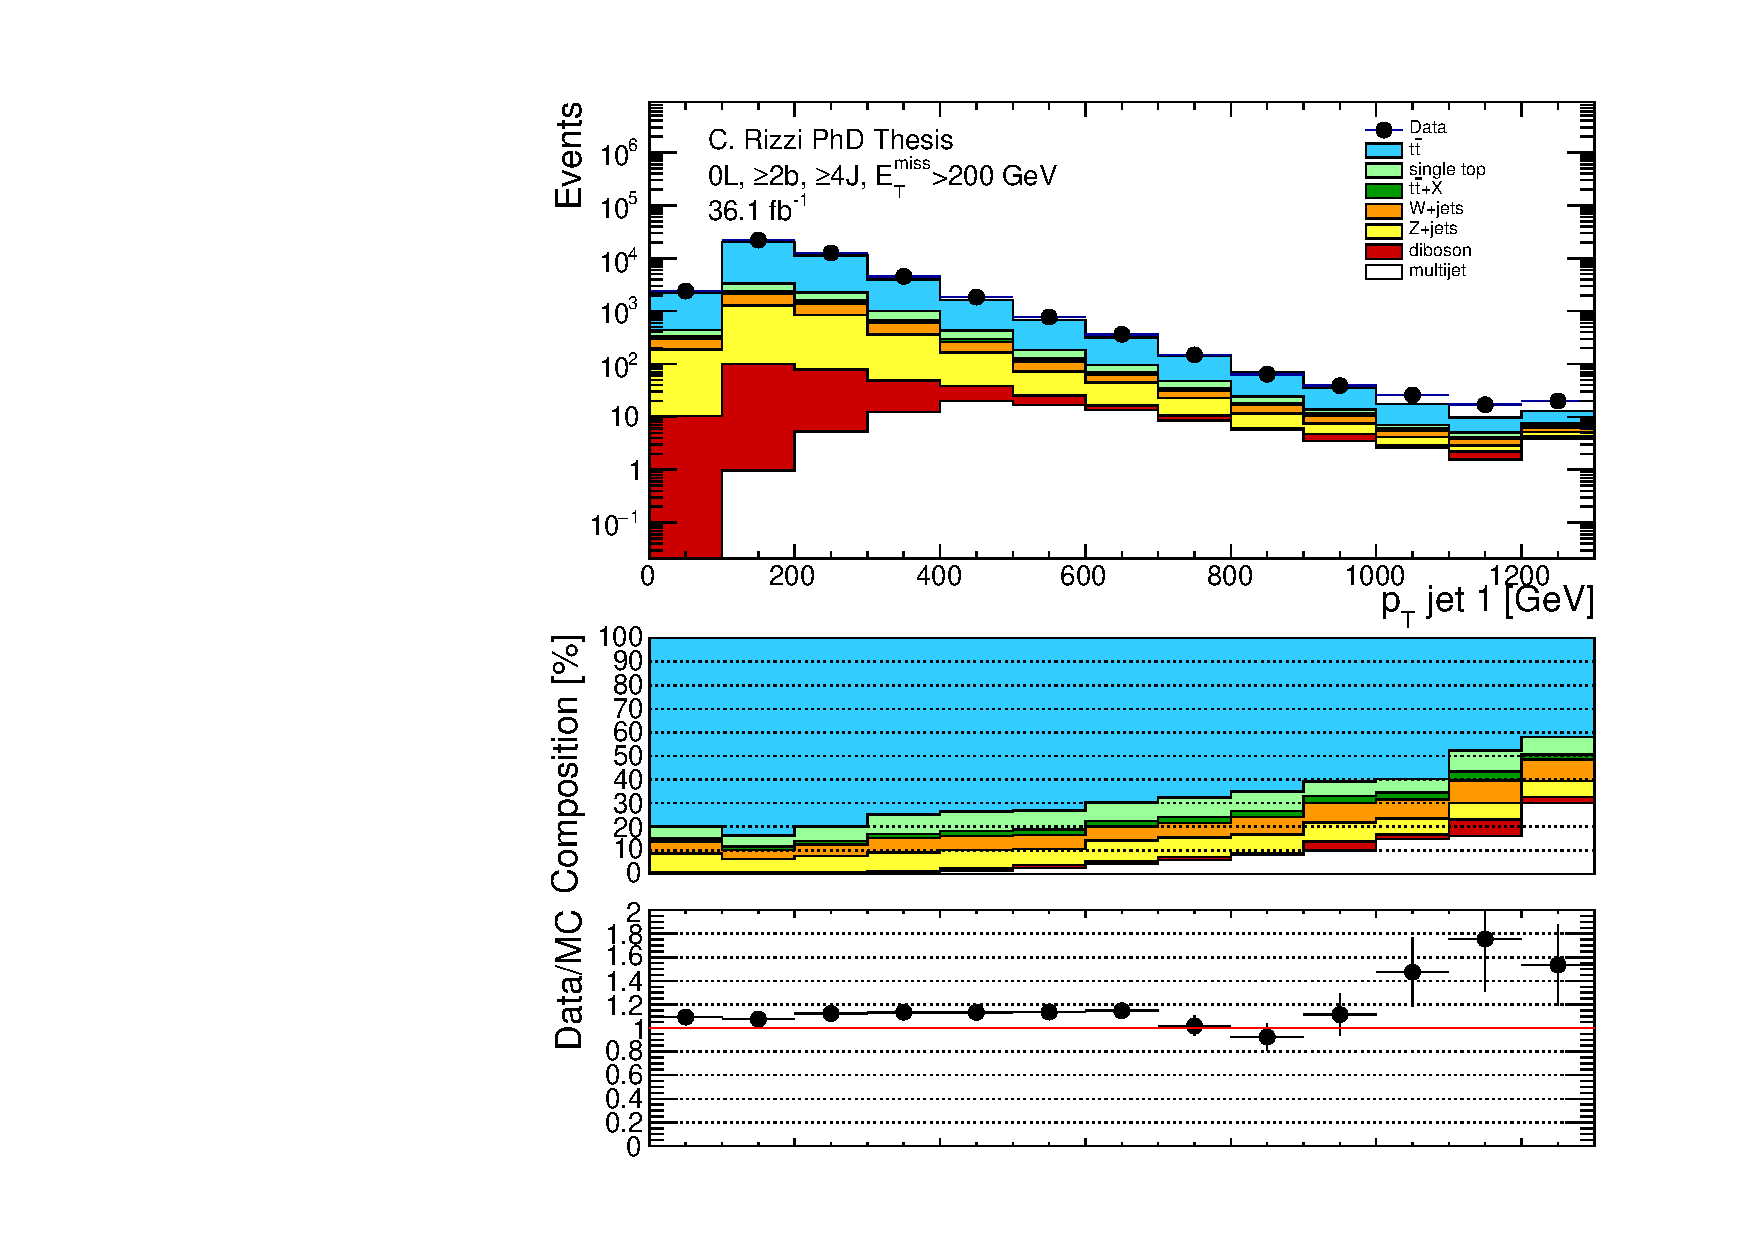
\includegraphics[width=0.4\textwidth]{figures/strong_prod/data_mc/0L_2bin/data_mc_pt_jet_1.pdf}
\label{fig:ewk:datamc0L:meff_incl}}
\subfigure[\met]{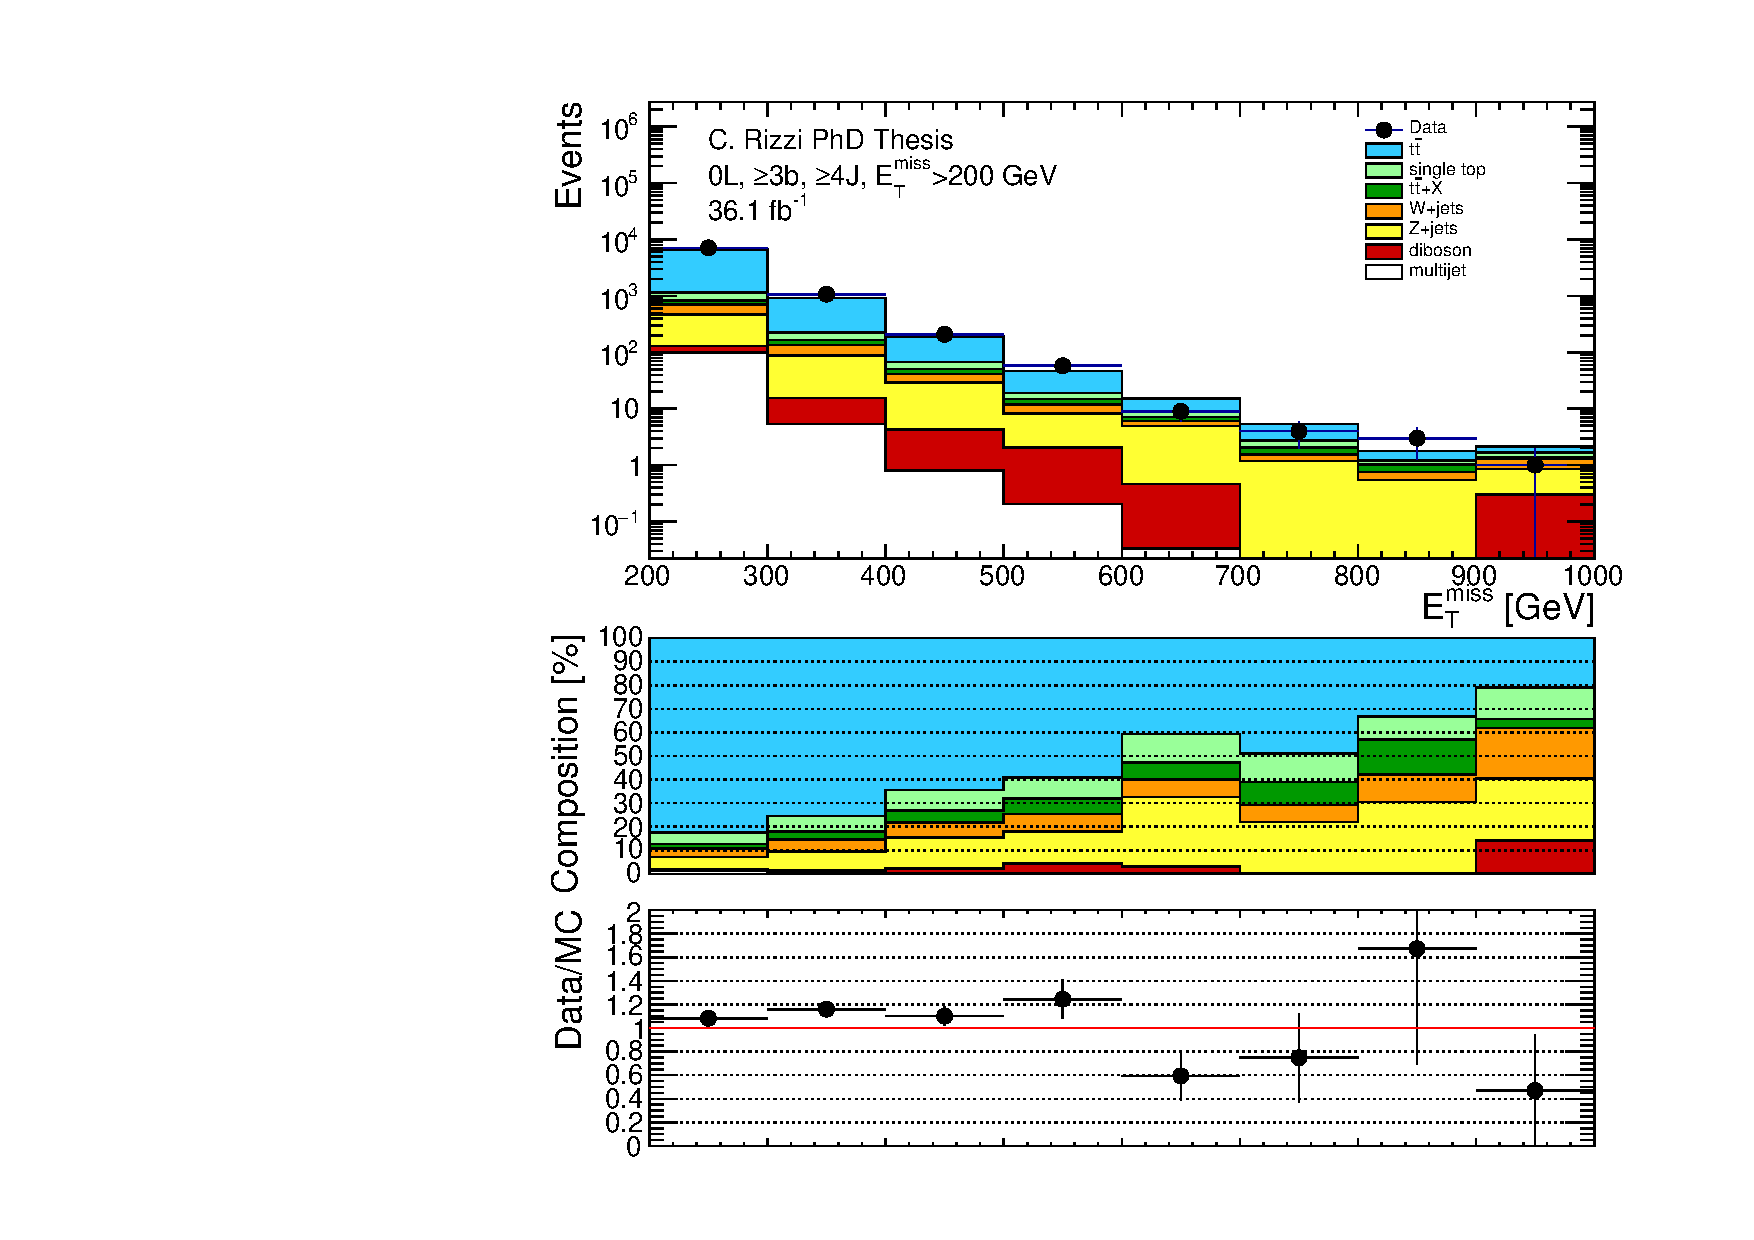
\includegraphics[width=0.4\textwidth]{figures/ewk_prod/data_mc/0L_3bin/data_mc_met.pdf}
\label{fig:ewk:datamc0L:met}}\\
\subfigure[$\phi$(\met)]{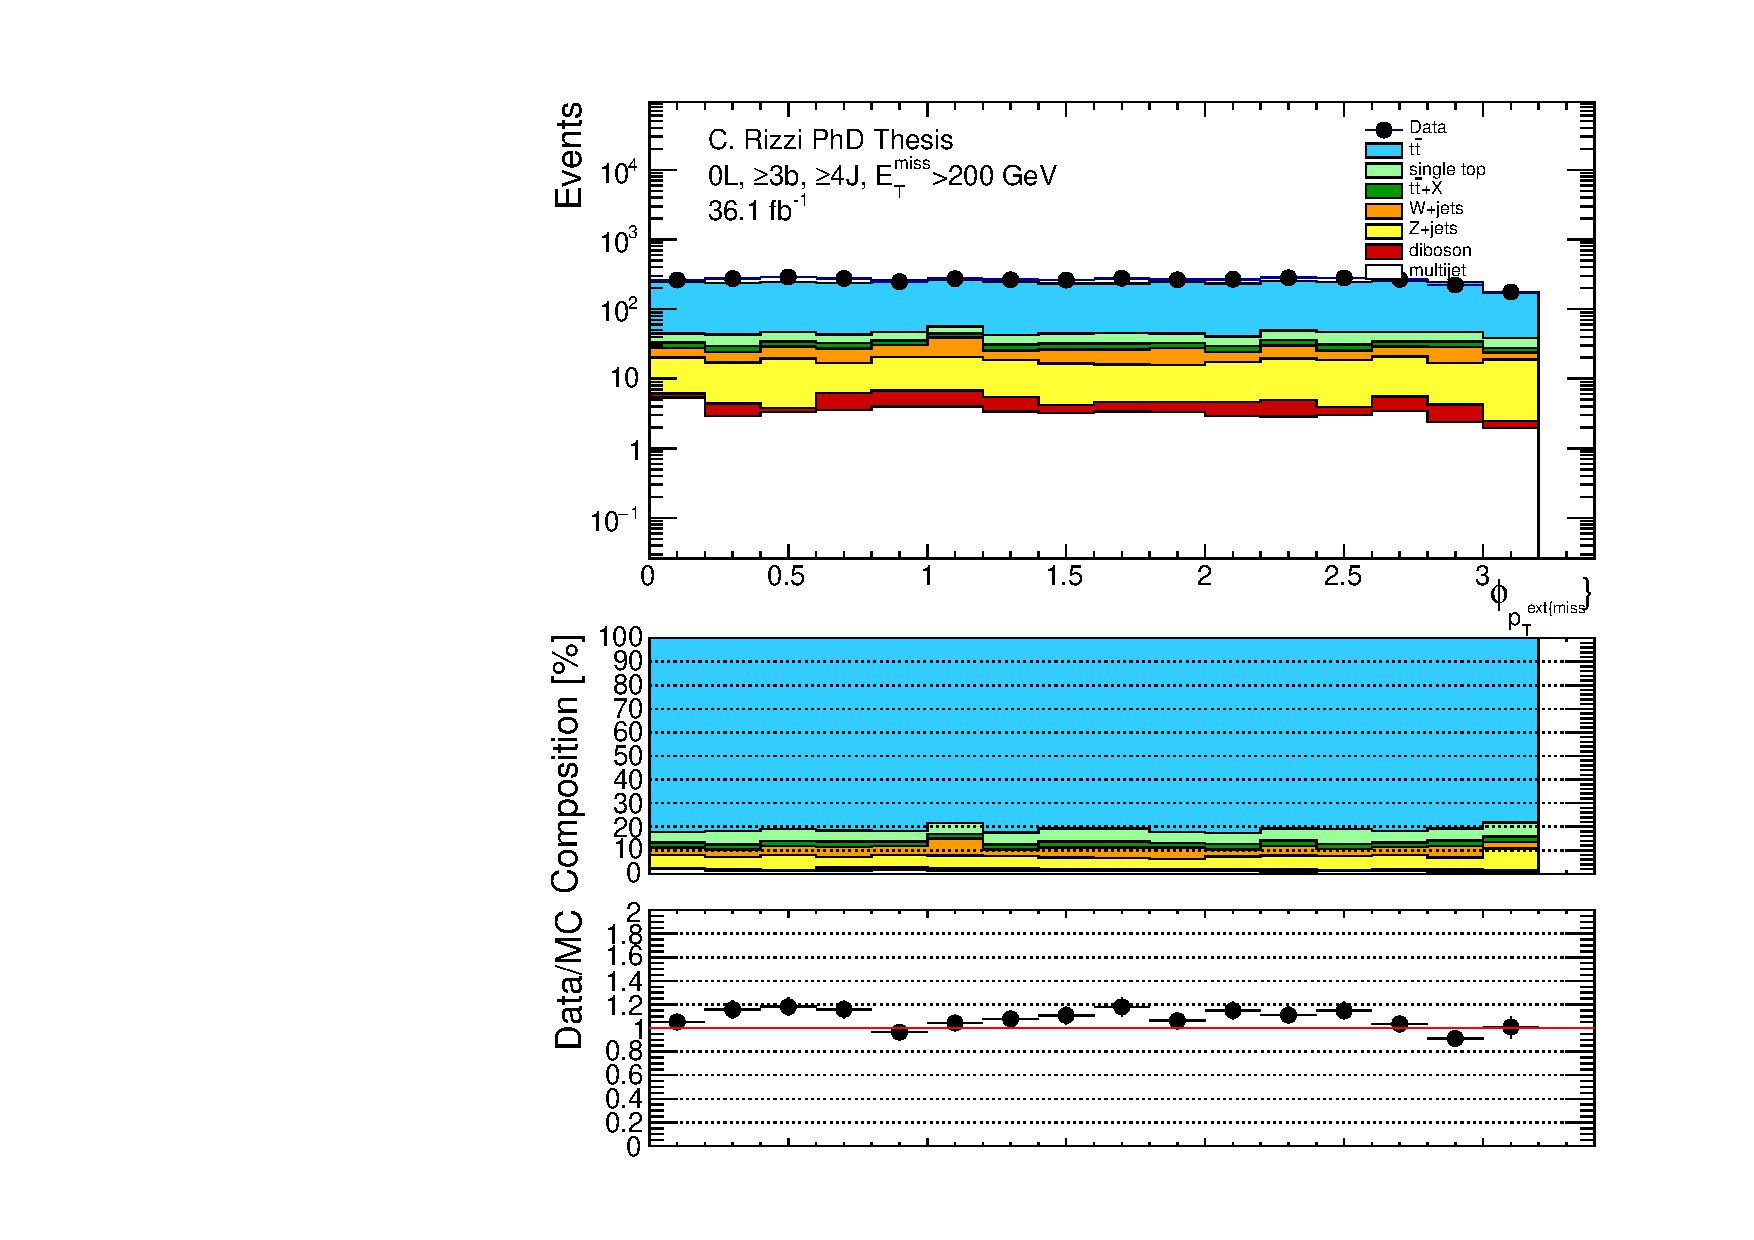
\includegraphics[width=0.4\textwidth]{figures/ewk_prod/data_mc/0L_3bin/data_mc_met_phi.pdf}
\label{fig:ewk:datamc0L:met_phi}}
\subfigure[\mt]{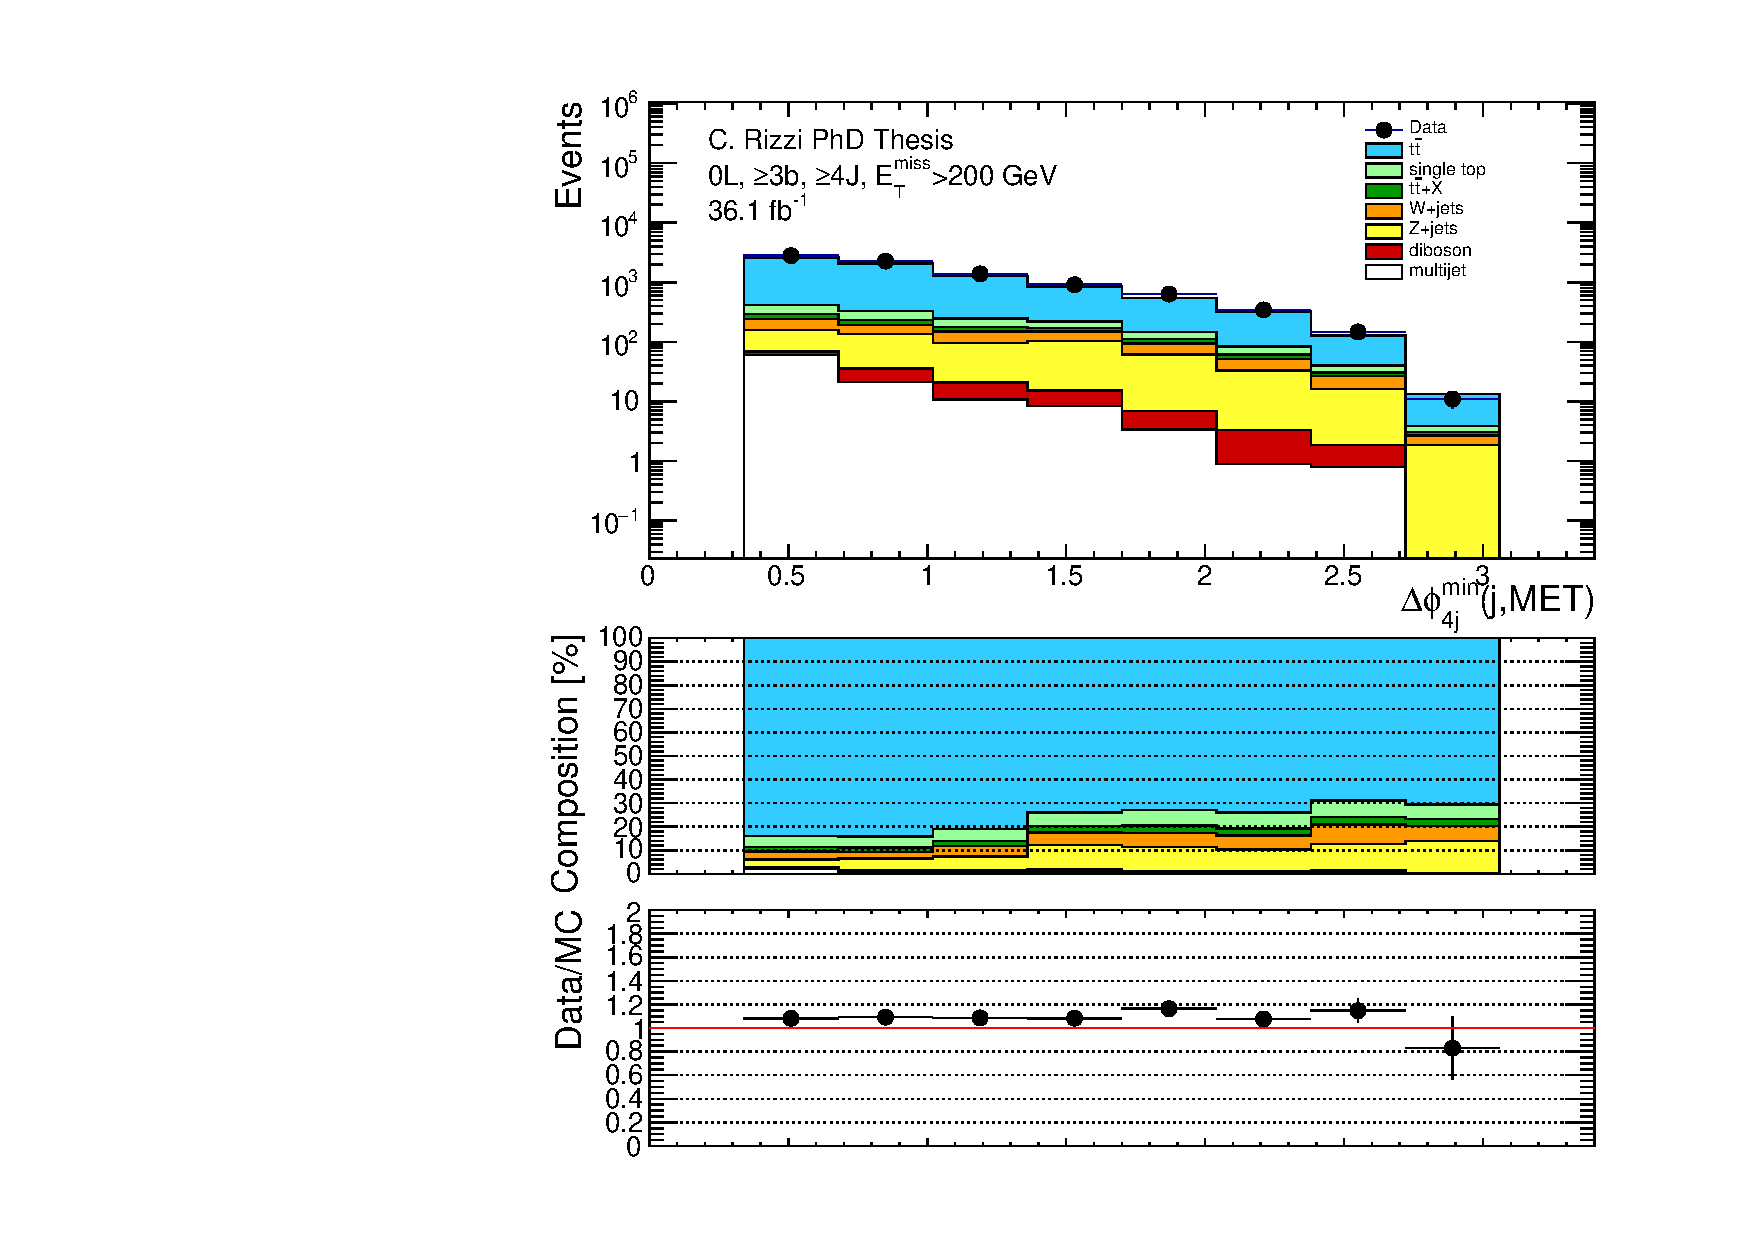
\includegraphics[width=0.4\textwidth]{figures/ewk_prod/data_mc/0L_3bin/data_mc_dphi_min.pdf}
\label{fig:ewk:datamc0L:mT}}\\
\subfigure[\mtb]{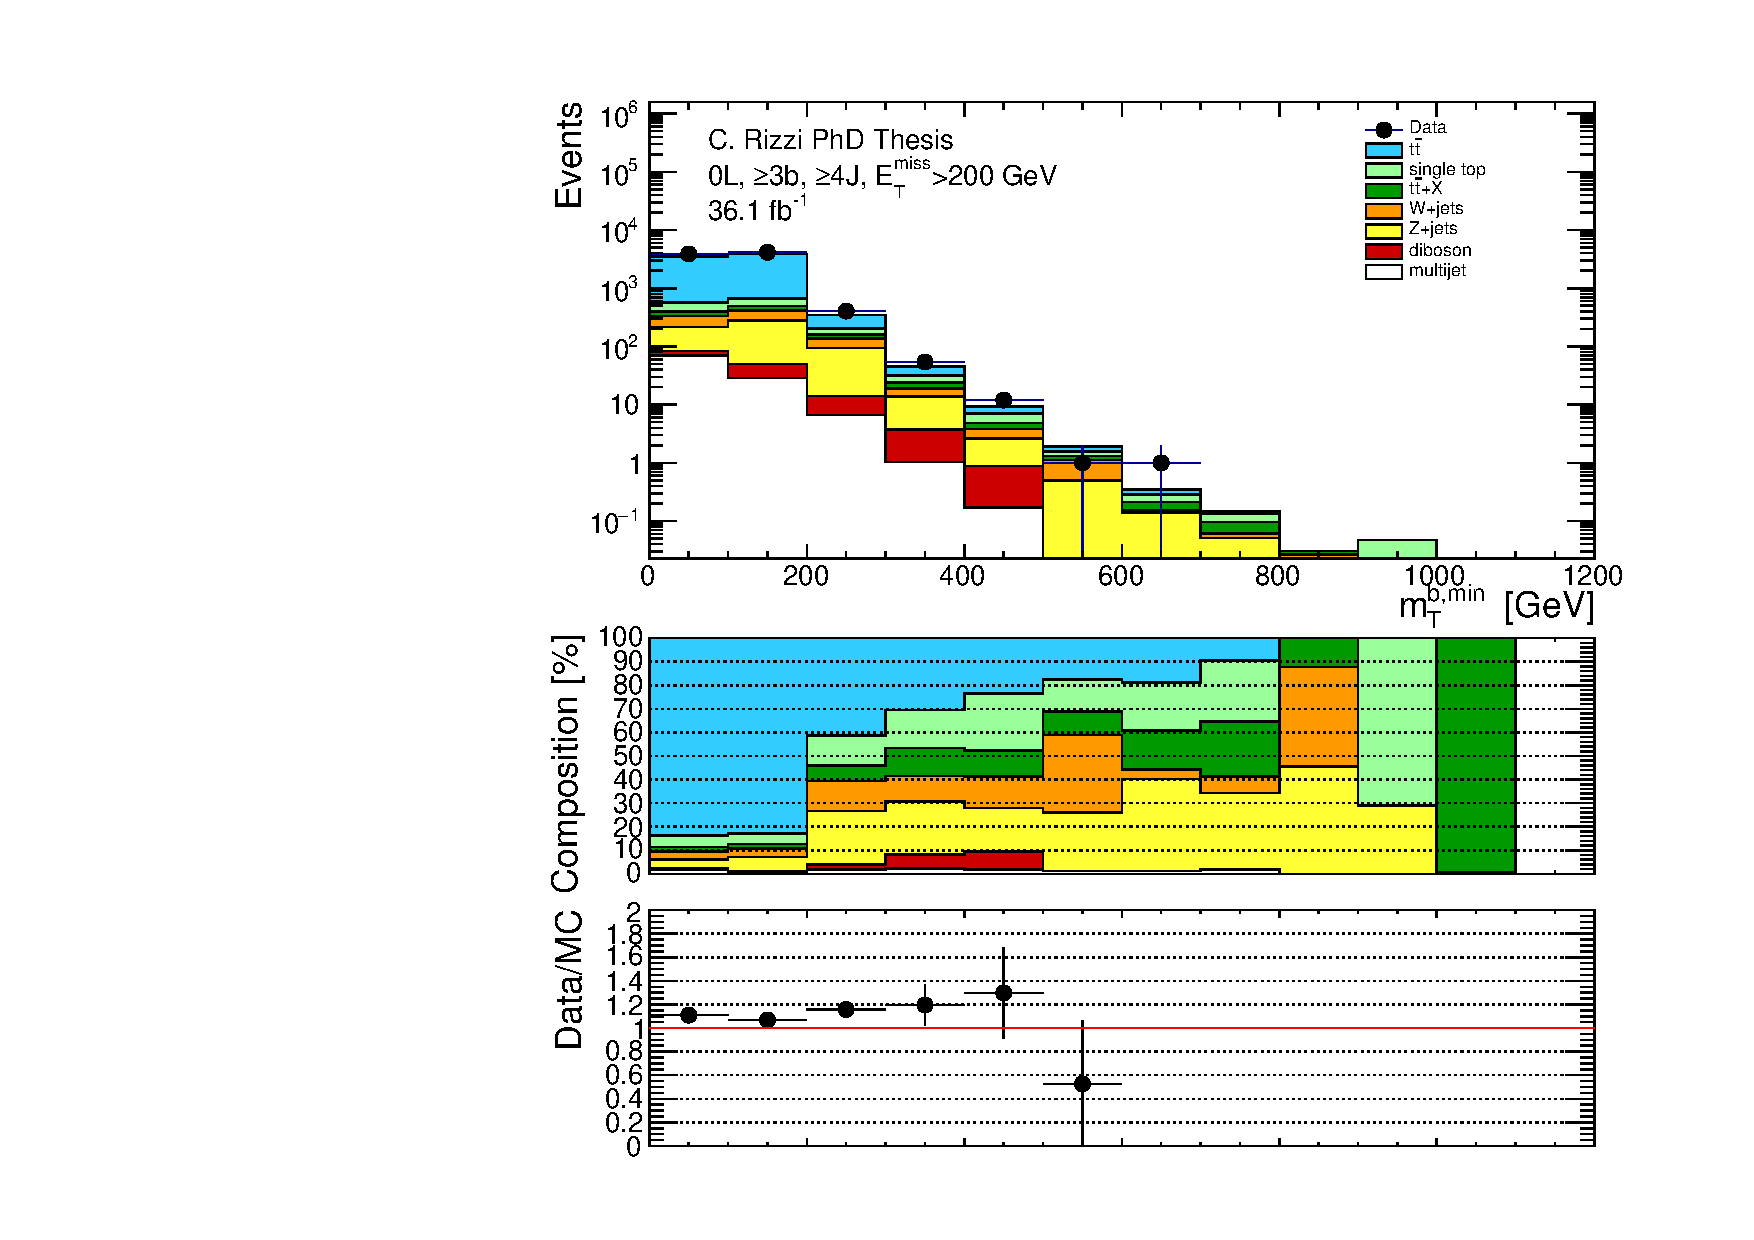
\includegraphics[width=0.4\textwidth]{figures/ewk_prod/data_mc/0L_3bin/data_mc_mTb_min.pdf}
\label{fig:ewk:datamc0L:mTb_min}}
\subfigure[\njet]{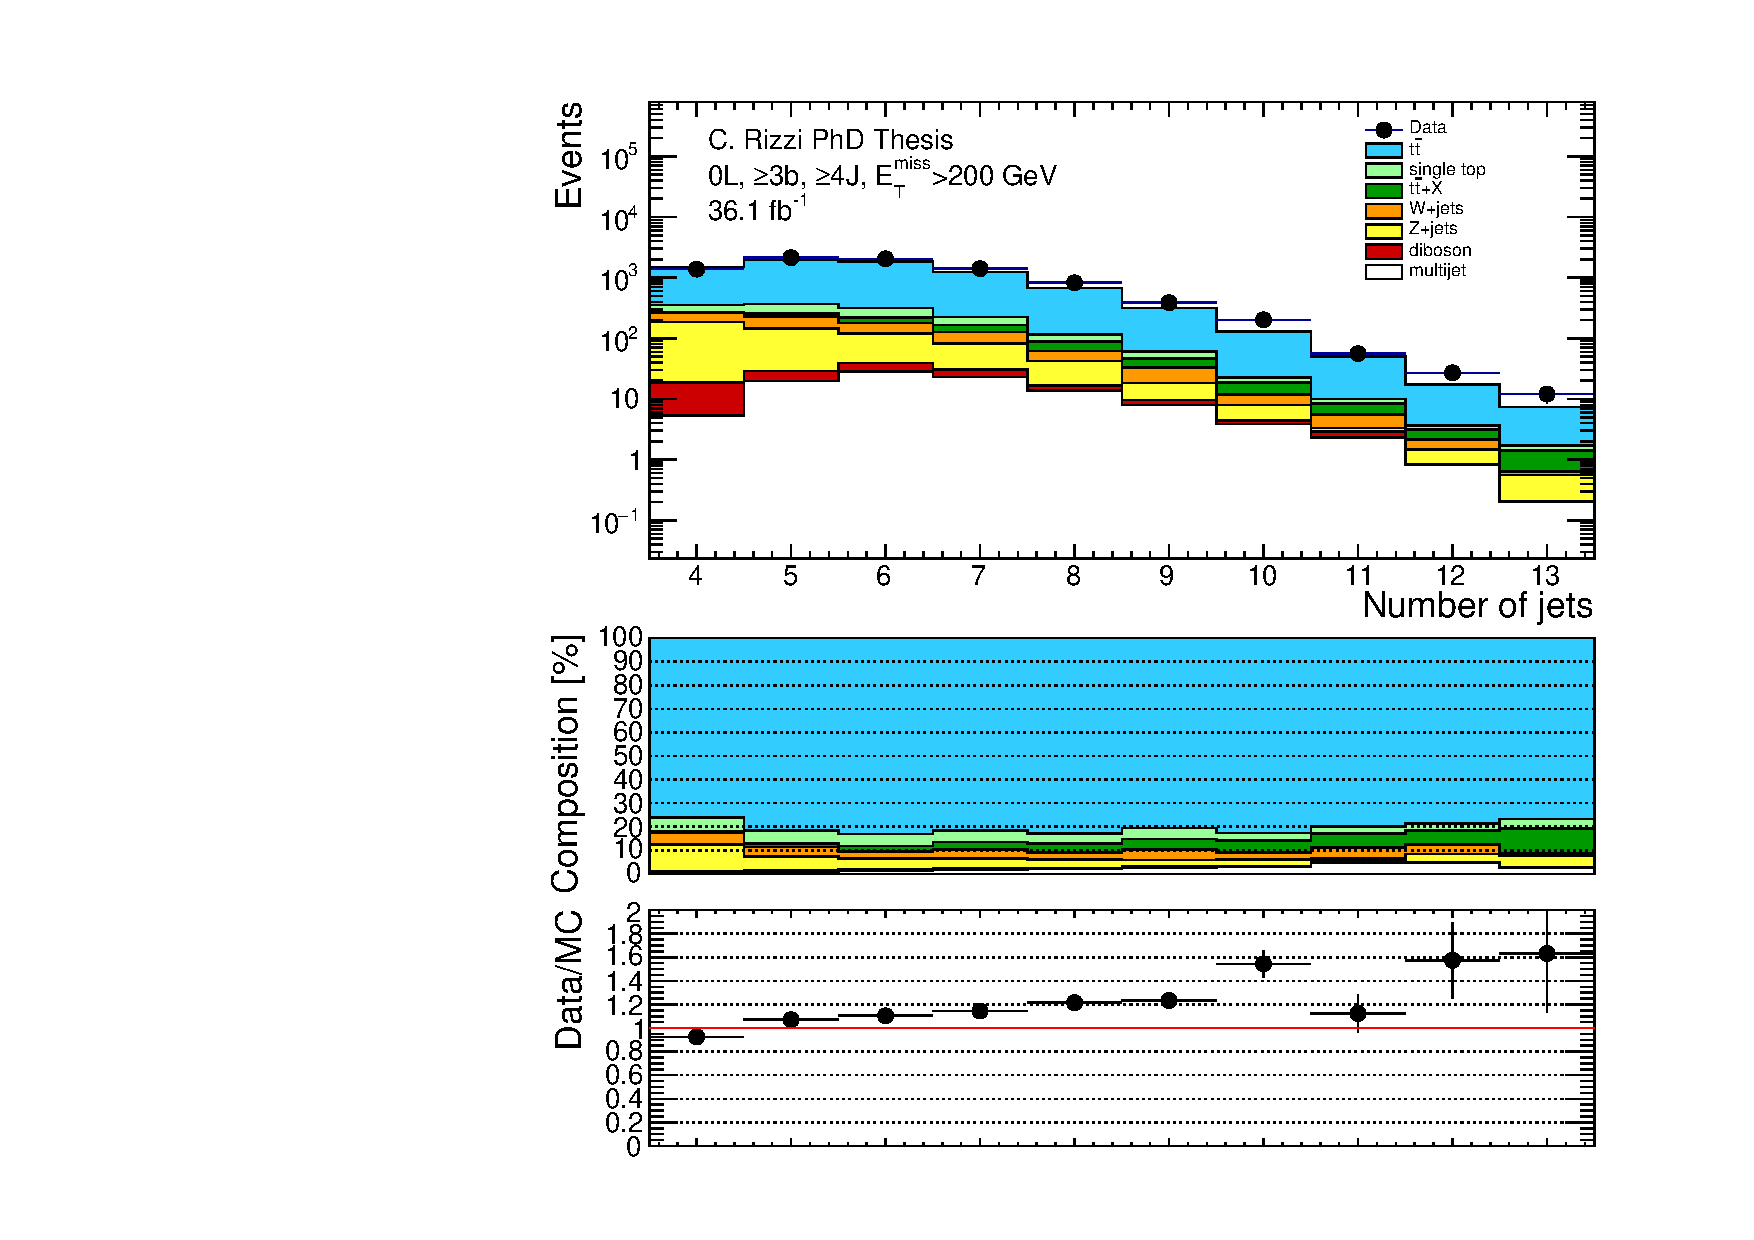
\includegraphics[width=0.4\textwidth]{figures/ewk_prod/data_mc/0L_3bin/data_mc_jets_n.pdf}
\label{fig:ewk:datamc0L:jets_n}}
\caption{Data-MC comparison in the 0-lepton preselection.
}
\label{fig:ewk:datamc0L_b}
\end{figure*}

